%\documentclass[wcp,gray]{jmlr} % test grayscale version
\documentclass[wcp]{jmlr}

% The following packages will be automatically loaded:
% amsmath, amssymb, natbib, graphicx, url, algorithm2e

%\usepackage{rotating}% for sideways figures and tables
\usepackage{longtable}% for long tables

% The booktabs package is used by this sample document
% (it provides \toprule, \midrule and \bottomrule).
% Remove the next line if you don't require it.
\usepackage{booktabs}
% The siunitx package is used by this sample document
% to align numbers in a column by their decimal point.
% Remove the next line if you don't require it.
%\usepackage[load-configurations=version-1]{siunitx} % newer version
%\usepackage{siunitx}

% The following command is just for this sample document:
\newcommand{\cs}[1]{\texttt{\char`\\#1}}

% This is required for dmath (display math)
\usepackage{breqn}

% To use multirow feature in table
\usepackage{multirow}

\jmlrvolume{29}
\jmlryear{2013}
\jmlrworkshop{ACML 2013}

\title[MML Laplace]{Minimum Message Length Estimate of Parameters of Laplace Distribution}

 % Use \Name{Author Name} to specify the name.
 % If the surname contains spaces, enclose the surname
 % in braces, e.g. \Name{John {Smith Jones}} similarly
 % if the name has a "von" part, e.g \Name{Jane {de Winter}}.
 % If the first letter in the forenames is a diacritic
 % enclose the diacritic in braces, e.g. \Name{{\'E}louise Smith}

 % Two authors with the same address
 % \author{\Name{Author Name1} \Email{abc@sample.com}\and
 %  \Name{Author Name2} \Email{xyz@sample.com}\\
 %  \addr Address}

 % Three or more authors with the same address:
 % \author{\Name{Author Name1} \Email{an1@sample.com}\\
 %  \Name{Author Name2} \Email{an2@sample.com}\\
 %  \Name{Author Name3} \Email{an3@sample.com}\\
 %  \Name{Author Name4} \Email{an4@sample.com}\\
 %  \Name{Author Name5} \Email{an5@sample.com}\\
 %  \Name{Author Name6} \Email{an6@sample.com}\\
 %  \Name{Author Name7} \Email{an7@sample.com}\\
 %  \Name{Author Name8} \Email{an8@sample.com}\\
 %  \Name{Author Name9} \Email{an9@sample.com}\\
 %  \Name{Author Name10} \Email{an10@sample.com}\\
 %  \Name{Author Name11} \Email{an11@sample.com}\\
 %  \Name{Author Name12} \Email{an12@sample.com}\\
 %  \Name{Author Name13} \Email{an13@sample.com}\\
 %  \Name{Author Name14} \Email{an14@sample.com}\\
 %  \addr Address}


 % Authors with different addresses:
  \author{\Name{Parthan Kasarapu} \Email{parthan.kasarapu@monash.edu}\\
  \addr Faculty of IT, Monash University, Clayton, VIC 3800, Australia
  \AND
  \Name{Lloyd Allison} \Email{lloyd.allison@monash.edu}\\
  \addr Faculty of IT, Monash University, Clayton, VIC 3800, Australia
  \AND
  \Name{Enes Makalic} \Email{emakalic@unimelb.edu.au}\\
  \addr Centre for MEGA Epidemiology, The University of Melbourne, Carlton, VIC 3053, Australia
 }

\editor{Cheng Soon Ong and Tu Bao Ho}
% \editors{List of editors' names}

\begin{document}

\maketitle

\begin{abstract}
The Laplace distribution offers a number of uses in statistical inference and
modelling of symmetric data with long tails. We report here for the first time
the derivation of the minimum message length (MML) estimates of location ($\mu$) and 
scale ($b$) parameters of the Laplace distribution for any observed data. 
We demonstrate an application of this work to compare and contrast the
quality of orthogonal superposition of two (spatial) vector sets under 
$\ell_1$ and $\ell_2$ norms.
\end{abstract}

\begin{keywords}
Laplace distribution, Normal distribution, minimum length encoding 
\end{keywords}

\section{Introduction}
The Laplace distribution is a continuous probability density function that is dependent on
the absolute value of the difference between the mean and the data point \textit{i.e.,}
the negative log probability varies linearly with the absolute difference. Because of
this characteristic, the inference of parameters of this distribution (based on some 
empirical data) is not severely affected by outliers. The Laplace distribution
is the model of choice in areas as diverse as signal processing 
\citep{laplace-signal-processing}, image denoising \citep{image-denoising},
gene expression studies \citep{Bhowmick01102006}, market risk prediction
\citep{haas2005modeling}, and machine learning \citep{Cord:2006:FSR:1167556.1167570}.
In most of these applications, a mixture model of Laplace distributions is used. 

The normal distribution, on the other hand, is sensitive to outliers because of the quadratic 
nature of the contributions of individual terms. 
In many problems, formulating an objective function (that needs 
to be optimized) as the sum of squared deviations (the $\ell_2$ norm) results in a closed
form solution. Its $\ell_1$ equivalent, however, does not have an analytical solution
(for data with more than one dimension). As such, one needs to adopt approximate 
methods to find the best superposition corresponding to the $\ell_1$ norm. 
We show this in the context of the superposition of vector sets and use a Monte Carlo simulation
to optimize the objective function when it is formulated using the $\ell_1$ norm. To compare
the superpositions obtained when using these two objective functions, we use
the minimum message length (MML) criterion. MML is used to adjudicate which is 
better on individual test cases. 

MML is an information theoretic method of Bayesian inference \citep{wallace68}. MML is best
understood through a communication process between an imaginary transmitter
and receiver connected over a Shannon channel. The method involves
encoding the model and its fit to the data. A model that results in the smallest total message
length is inferred as the most suitable under this criterion. Indeed the message length
paradigm provides an objective means to differentiate between competing models
and select the best one. In this paper, we use this technique to 
evaluate the overall fit when the data is modelled  using a Normal and a Laplace distribution. 

While the MML expression for the Normal distribution has been 
worked out previously \citep{wallace68,WallaceBook}, the MML estimates for the Laplace 
distribution have not been characterized. 
The main contribution of our work is the derivation of the message length 
expression and estimation of the MML parameters for the Laplace distribution.
The general procedure to formulate the message length expression for transmitting
data using some statistical model is outlined in \citet{wallace-75} and is 
referred to as Strict Message Length (SMML) Inference. This is computationally
infeasible and is shown to be NP-hard for most models \citep{Farr01012002}. 
\citet{wallace-87} provide a quadratic approximation which is often easy to compute
and is commonly referred to as the \emph{Wallace-Freeman} approximation. The MML method
of estimating parameters for a number of distributions using this approximation
has been well established \citep{WallaceBook}. In this paper, we use the 
Wallace--Freeman quadratic approximation
to derive the message length expression for the Laplace distribution. 

The results demonstrate the use of Laplace estimates in two cases. 
The first scenario involves data being randomly
generated from a Laplace distribution. This data is then fitted using
both Normal and Laplace models. We use the derived formulation of Laplace MML to
compute the Laplace fit. This is then compared against the fit using a Normal
distribution. 

As a demonstration of a practical real world application, we consider the problem of
superposition of vector sets. The objective function for the superposition problem can be formulated
where the deviations of the corresponding vectors are calculated using the $\ell_1$ norm 
or the $\ell_2$ norm. In MML parlance, the optimal superposition would correspond to stating
the deviations concisely. We encode the deviations using both Normal and Laplace
distributions. The distribution which results in the best compression is chosen
to be the best model for those two vector sets.

\section{The Minimum Message Length (MML) Framework}
\subsection{Inductive Inference}
\citet{wallace68} developed the first practical criterion for model selection using 
information theory. MML provides an elegant framework to compare any competing 
hypotheses that model some observed data. As mentioned before, the hypothesis that results in the shortest 
overall message length is chosen as the best one, in line with traditional statistical 
inference using the Bayesian method\footnote{http://allisons.org/ll/MML/} which maximizes
the posterior distribution of the parameters given the data.
Using Bayes's theorem to explain some observed data $D$ by hypothesis $H$, we get:
$$\Pr(H\&D) = \Pr(H) \times \Pr(D|H) = \Pr(D) \times \Pr(H|D)$$
where $\Pr(H\&D)$ is the joint probability of data $D$ and hypothesis $H$, $\Pr(H)$
is the prior probability of hypothesis $H$, $\Pr(D)$ is the prior 
probability of data $D$, $\Pr(H|D)$ is the posterior probability of $H$
given $D$, and $\Pr(D|H)$ is the likelihood.
MML uses the following result from information theory: given an event $E$
with a probability $\Pr(E)$, the message length $I(E)$ for an optimal
code is given by $I(E) = -\log_2 (\Pr(E))$ bits \citep{shannon1948}. Applying this insight
to the Bayes's theorem, we get the following relationship between
conditional probabilities in terms of optimal message lengths:\[I(H\&D) = I(H) + I(D|H) = I(D) + I(H|D)\]
In the traditional Bayesian framework, the hypothesis $H$ with
the largest posterior probability $\Pr(H|D)$ is often preferred.
Among the terms in the above equation, $\Pr(H)$ (and hence $I(H)$) can
usually be estimated well for some \emph{reasonable} prior(s) on hypotheses.
Given the data $D$ and a chosen prior $H$, the likelihood $\Pr(D|H)$ can also be estimated.
When comparing competing hypotheses, the prior of observed data $\Pr(D)$
can be ignored as it is a common factor. Hence, for two competing hypotheses, $H$ and $H^\prime$, we have:
$$I(H|D) - I(H^\prime|D) = I(H) + I(D|H) - I(H^\prime) - I(D|H^\prime)$$
The discriminative ability of MML lies in its consideration of the model
complexity and the error of the fit. In the MML setting, the total message length,
therefore, involves a statement cost of the hypothesis
(given by $I(H)$) and a statement cost of the data given the hypothesis (given by $I(D|H)$). 

\subsection{Parameter Estimation using MML}
The hypothesis is a statistical model which is characterized by its parameters.
MML accounts for both the model complexity and its explanatory power of the 
data observed. MML works by maximizing the expectation of the posterior
probability and this is where it differs from the traditional Bayesian methods.
This involves determining the \emph{accuracy of parameter values (AOPV)} for
continuous parameters. AOPV is a measure of the uncertainty in stating a
parameter and it is this region over which the expectation is maximized. As per
MML, a parameter need not be stated very accurately. The optimal precision to which
it needs to be stated is computed as part of the MML inference. A good
description of the procedure is outlined in \citet{oliver1994mml}. 

\section{Message Length of Laplace distribution}
\citet{wallace-87} derived the approximation to the code length of the two part message as
\begin{align}
I(\bar{\theta},D) &= I(\bar{\theta}) + I(D|\bar{\theta}) \notag\\
&\approx \underbrace{\frac{d}{2}\log\kappa_d -\log h(\bar{\theta}) + \frac{1}{2}\log(det\,F(\bar{\theta}))}_{\mathrm{part 1}} + \underbrace{L(\bar{\theta}) + \frac{d}{2}}_{\mathrm{part 2}} \label{eqn:wf_msglen}
\end{align}
where $\bar{\theta}$ is the set of model parameters, $d$ is the number of parameters, 
$\kappa_d$ is the $d$-dimensional lattice quantization constant \citep{conwaySloane84}, 
$h(\bar{\theta})$ is the prior probability of the parameters, 
$det(\mathrm{F}(\bar{\theta}))$ is the determinant of the expected Fisher matrix, and
$\ell(\bar{\theta})$ is the negative log likelihood of observed data. The MML estimates 
$\hat{\bar{\theta}}_{\mathrm{MML}}$ of the parameters are determined by minimizing 
expression \eqref{eqn:wf_msglen}. 

\subsection{Laplace distribution}
The contribution of this paper is in the derivation of the MML estimates of 
the parameters of the Laplace distribution which have not been characterized previously.
The parameters describing a Laplace distribution are the location($\mu$) and the scale ($b$).
The probability density function (pdf) is given in \eqref{eqn:laplace_pdf}.
\begin{equation}
\mathrm{pdf}(x) = \frac{1}{2b}e^{-\frac{|x-\mu|}{b}} \label{eqn:laplace_pdf}
\end{equation}
To derive the MML estimates, we use the Wallace--Freeman approximation. 
This estimation as per \eqref{eqn:wf_msglen} requires the likelihood function, the Fisher information matrix,
and the prior distributions on the parameters. Let $D = \{x_1,x_2,\ldots,x_N\}$ be the observed data 
containing $N$ samples and $\epsilon$ be the precision to which each datum is stated. 
Let $\mathrm{R}_{\mu}$, $\mathrm{R}_{b}$ be the range of $\mu$ and $\log b$ 
respectively. $\epsilon$, $\mathrm{R}_{\mu}$, $\mathrm{R}_{b}$ are hyperparameters
introduced in \citet{WallaceBook}. These are fixed and will
not be inferred from the observed data. 
Using \autoref{eqn:laplace_pdf}, the \emph{likelihood function} is given by
\[ f(D|\bar{\theta}) = \prod_{n=1}^N \frac{\epsilon}{2b} e^{-\frac{|x_n-\mu|}{b}} \]
and, hence, the \emph{negative log-likelihood} is computed as
\begin{align}
 L(\bar{\theta}) &= -\log f(D|\bar{\theta}) \notag\\
		 &= N\log\left(\frac{2}{\epsilon}\right) + N\log b + \frac{1}{b}\sum_{n=1}^N |x_n-\mu| \label{eqn:laplace_l}
\end{align}
The maximum likelihood (ML) estimates for $\mu$ and $b$ are given by
\begin{align}
\hat{\mu}_{\mathrm{ML}} &= \mathrm{median}\{x_1,x_2,\ldots,x_n\} \notag\\ 
\hat{b}_{\mathrm{ML}} &= \frac{1}{N} \sum_{n=1}^N |x_n-\hat{\mu}_{\mathrm{ML}}| \label{eqn:ml_estimate}
\end{align}

\subsection*{Computation of Fisher information $\mathbf{F(\bar{\boldsymbol{\theta}})}$}
The Fisher information matrix is given by
\begin{align*}
  \mathrm{F}(\mu,b) &= \left( \begin{array}{cc}
  \mathrm{E} \left[\frac{\partial^2 L}{\partial \mu^2}\right] & \mathrm{E} \left[\frac{\partial^2 L}{\partial\mu \partial b}\right] \\
  \mathrm{E} \left[\frac{\partial^2 L}{\partial b \partial\mu}\right] & \mathrm{E} \left[\frac{\partial^2 L}{\partial b^2}\right] 
  \end{array} \right) 
\end{align*}
where $\mathrm{E}[.]$ is the expected value of that quantity. Using \autoref{eqn:laplace_l}, we have:
\begin{align*}
 \frac{\partial^2 L}{\partial b^2} &= -\frac{N}{b^2} + \frac{2}{b^3} \sum_{n=1}^N |x_n-\mu| \\
 \mathrm{E} \left[\frac{\partial^2 L}{\partial b^2}\right] &= -\frac{N}{b^2} + \frac{2}{b^3} \mathrm{E}\left[\sum_{n=1}^N |x_n-\mu|\right]
\end{align*}
\begin{align*}
 \mathrm{E}\left[|x-\mu|\right] &= \int\limits_{-\infty}^{\infty} |x-\mu| . \frac{1}{2b} . e^{-\frac{|x-\mu|}{b}} dx \\
 &= \frac{1}{2b} \int\limits_{-\infty}^{\mu} -(x-\mu) e^{\frac{(x-\mu)}{b}} dx + \int\limits_{\mu}^{\infty} (x-\mu)e^{-\frac{(x-\mu)}{b}} dx \\
 &= b
\end{align*}
\begin{equation}
 \mathrm{Therefore,}\quad \mathrm{E} \left[\frac{\partial^2 L}{\partial b^2}\right] = -\frac{N}{b^2} + \frac{2}{b^3} (Nb) = \frac{N}{b^2} \label{eqn:fisher_44} 
\end{equation}
The computation of $\mathrm{E}\left[\frac{\partial^2 L}{\partial \mu^2}\right]$ and 
$\mathrm{E}\left[\frac{\partial^2 L}{\partial \mu \partial b}\right]$ is involved and, hence,
discussed in \autoref{apd:laplace_fisher}. Using those results, we have
%\section{Derivations involved in the computation of Laplace Fisher}
%\label{apd:laplace_fisher}
%\begin{align*}
% \frac{\partial L}{\partial \mu} &= -\frac{1}{b} \sum_{n=1}^N \frac{(x_n-\mu)}{|x_n-\mu|} \quad\quad\left(\mathrm{using} \frac{d}{dx}|x| = \frac{d}{dx}\sqrt{x^2} = \frac{x}{|x|}\right)
%\end{align*}
%This is discontinuous as it is piecewise constant. Hence, to calculate $\frac{\partial^2 L}{\partial \mu^2}$, 
%the following approach is adopted. Assume that the actual distribution has parameters $m$ and 
%$b$. The receiver, however, decodes the mean as $\mu$ to an accuracy of parameter
%value $\delta$. As such $\mu$ is a random variable and it is fair to say
%that $\mu \in \left[m-\frac{\delta}{2},m+\frac{\delta}{2}\right]$. It is 
%assumed that $\mu$ follows a uniform distribution in this range. Using this 
%assumption, we now compute the $\mathrm{E}\left[\frac{\partial L}{\partial \mu}\right]$ 
%and subsequent calculations. From our assumptions, $\mathrm{pdf}(\mu) = \frac{1}{\delta}$.
%\begin{align*}
% \therefore \frac{\partial L}{\partial \mu} &\approx \mathrm{E}\left[\frac{\partial L}{\partial \mu}\right] = -\frac{1}{b}\mathrm{E}\left[\sum_{n=1}^{N}\frac{x_n-\mu}{|x_n-\mu|}\right]
%\end{align*}
%\begin{align*}
% \mathrm{E}\left[\frac{x-\mu}{|x-\mu|}\right] &= \int\limits_{-\infty}^{\infty} \frac{x-\mu}{|x-\mu|}.\frac{1}{2b}.e^{\frac{|x-m|}{b}} dx \\
% &= \int\limits_{-\infty}^{\mu} -\frac{1}{2b} e^{-\frac{|x-m|}{b}} dx + \int\limits_{\mu}^{\infty} \frac{1}{2b} e^{-\frac{|x-m|}{b}} dx
%\end{align*}
%(i) Let $\mu < m$
%\begin{align*}
% \therefore \mathrm{E}\left[\frac{x-\mu}{|x-\mu|}\right] &= \int\limits_{-\infty}^{\mu} -\frac{1}{2b} e^{\frac{x-m}{b}} dx + \int\limits_{\mu}^{m} \frac{1}{2b} e^{\frac{x-m}{b}} dx + \int\limits_{m}^{\infty} \frac{1}{2b} e^{-\frac{x-m}{b}} dx \\
% &= 1 - e^{\frac{\mu-m}{b}}
%\end{align*}
%(ii) Let $\mu > m$
%\begin{align*}
% \therefore \mathrm{E}\left[\frac{x-\mu}{|x-\mu|}\right] &= \int\limits_{-\infty}^{m} -\frac{1}{2b} e^{\frac{x-m}{b}} dx + \int\limits_{m}^{\mu} -\frac{1}{2b} e^{-\frac{x-m}{b}} dx + \int\limits_{\mu}^{\infty} \frac{1}{2b} e^{-\frac{x-m}{b}} dx \\
% &= -(1 - e^{-\frac{\mu-m}{b}})
%\end{align*}
%(i) and (ii) can be merged and hence, $\mathrm{E}\left[\frac{x-\mu}{|x-\mu|}\right] = - sgn(\mu-m) (1 - e^{-\frac{|\mu-m|}{b}})$. From the argument above,
%\begin{align}
% \frac{\partial L}{\partial \mu} &\approx \mathrm{E}\left[\frac{\partial L}{\partial \mu}\right] = -\frac{1}{b} \mathrm{E}\left[\sum_{n=1}^{N}\frac{x_n-\mu}{|x_n-\mu|}\right]\notag\\
% &= \frac{N}{b} sgn(\mu-m) (1 - e^{-\frac{|\mu-m|}{b}}) \label{eqn:laplace_expected_approx}\\
% \therefore \frac{\partial^2 L}{\partial \mu^2} &= \frac{N}{b^2} e^{\frac{-|\mu-m|}{b}} \notag\\
% \mathrm{E} \left[\frac{\partial^2 L}{\partial \mu^2}\right] &= \frac{N}{b^2} \mathrm{E}\left[e^{\frac{-|\mu-m|}{b}}\right] \notag
%\end{align}
%\begin{align*}
% \mathrm{E}\left[e^{\frac{-|\mu-m|}{b}}\right] &= \int\limits_{m-\frac{\delta}{2}}^{m+\frac{\delta}{2}} e^{\frac{-|\mu-m|}{b}} . \frac{1}{\delta} . d\mu \\
% &= \frac{1}{\delta} \int\limits_{m-\frac{\delta}{2}}^{m} e^{\frac{\mu-m}{b}} d\mu + \int\limits_{m}^{m+\frac{\delta}{2}}e^{-\frac{\mu-m}{b}} d\mu \\
% &= 2b \left(\frac{1-e^{-\frac{\delta}{2b}}}{\delta}\right) \\
% &= 2b \left( \frac{1}{2b} - \frac{1}{2b}\mathcal{O}\left(\frac{\delta}{2b}\right) \right) \quad\quad(\mathrm{assuming} \quad \delta \ll 2b) \\
% &\approx 1
% \end{align*}
%\begin{equation}
% \mathrm{Therefore,}\quad \mathrm{E} \left[\frac{\partial^2 L}{\partial \mu^2}\right] = \frac{N}{b^2} (1) = \frac{N}{b^2} \label{eqn:fisher_11}
%\end{equation}
%Using \eqref{eqn:laplace_expected_approx}, 
%\begin{align*}
% \frac{\partial^2 L}{\partial b \partial \mu} &= N sgn(\mu-m) \left[ -\frac{1}{b^2} - \left( e^{\frac{-|\mu-m|}{b}} \left( -\frac{1}{b^2} \right) + \frac{1}{b} e^{\frac{-|\mu-m|}{b}} \frac{|\mu-m|}{b^2} \right) \right] \\
% &= -\frac{N}{b^2} sgn(\mu-m)(1-e^{-\frac{|\mu-m|}{b}}) - \frac{N}{b} . \frac{(\mu-m)}{b^2} . e^{-\frac{|\mu-m|}{b}} \\
% \mathrm{Therefore,}\quad \mathrm{E} \left[\frac{\partial^2 L}{\partial b \partial \mu}\right] &= -\frac{N}{b^2} (\mathrm{E}_1 - \mathrm{E}_2) - \frac{N}{b^3} \mathrm{E}_3, \quad\quad\mathrm{where}
%\end{align*}
%\begin{align*}
% \mathrm{E}_1 &= \mathrm{E}[sgn(\mu-m)] = \int\limits_{m-\frac{\delta}{2}}^{m+\frac{\delta}{2}} sgn(\mu-m).\frac{1}{\delta}.d\mu = \frac{1}{\delta} \int\limits_{m-\frac{\delta}{2}}^{m+\frac{\delta}{2}} \frac{\mu-m}{|\mu-m|} d\mu \\
% &= \frac{1}{\delta} \int\limits_{-\frac{\delta}{2}}^{\frac{\delta}{2}} \frac{t}{|t|} dt = 0 \quad\quad(\mathrm{as\,\,the\,\,integrand\,\,is\,\,an\,\,odd\,\,function})
%\end{align*}
%\begin{align*}
% \mathrm{E}_2 &= \mathrm{E}[sgn(\mu-m)e^{-\frac{|\mu-m|}{b}}] = \frac{1}{\delta} \int\limits_{m-\frac{\delta}{2}}^{m+\frac{\delta}{2}} \frac{\mu-m}{|\mu-m|} e^{-\frac{|\mu-m|}{b}} d\mu \\
% &= \frac{b}{\delta} \int\limits_{-\frac{\delta}{2}}^{\frac{\delta}{2}} \frac{t}{|t|} e^{-|t|} dt = 0 \quad\quad(\mathrm{as\,\,the\,\,integrand\,\,is\,\,an\,\,odd\,\,function})
%\end{align*}
%\begin{align*}
% \mathrm{E}_3 &= \mathrm{E}[(\mu-m)e^{-\frac{|\mu-m|}{b}}] = \frac{1}{\delta} \int\limits_{m-\frac{\delta}{2}}^{m+\frac{\delta}{2}} (\mu-m)e^{-\frac{|\mu-m|}{b}} d\mu \\
% &= \frac{b^2}{\delta} \int\limits_{-\frac{\delta}{2}}^{\frac{\delta}{2}} t e^{-|t|} dt = 0 \quad\quad(\mathrm{as\,\,the\,\,integrand\,\,is\,\,an\,\,odd\,\,function})
%\end{align*}
%\begin{equation} 
%  \mathrm{Therefore,}\quad \mathrm{E} \left[\frac{\partial^2 L}{\partial b \partial \mu}\right] = 0 \label{eqn:fisher_22} 
%\end{equation}
%Using \eqref{eqn:fisher_44}, \eqref{eqn:fisher_11}, \eqref{eqn:fisher_22},
\begin{align*}
  \mathrm{F}(\mu,b) &= \left( \begin{array}{cc}
        \frac{N}{b^2} & 0 \\
        0 & \frac{N}{b^2}
            \end{array} \right) 
\end{align*}
\begin{equation} \mathrm{Therefore,}\quad det(\mathrm{F}(\mu,b)) = \frac{N^2}{b^4} \label{eqn:laplace_fisher} \end{equation}

\subsection*{Priors on the parameters}
A prior probability on $\mu$ and $b$ is assumed in accordance with the prior assumed
in the case of Normal. It is assumed that $\mu$ and $b$ have independent priors,
that $\mu$ has a uniform prior density (location invariance), and that $\log b$
has a uniform prior density (scale invariance) \citep{WallaceBook}.
The ranges from which $\mu$ and $\log b$ are drawn are assumed to be 
$\mathrm{R}_{\mu}$ and $\mathrm{R}_{b}$ respectively. The joint prior probability
of the parameters is then given by
\begin{align} 
  h(\bar{\theta}) = h(\mu,b) &= h(\mu) h(b) \notag\\
      &= \frac{1}{\mathrm{R}_{\mu}}. \frac{1}{b \mathrm{R}_{b}} \label{eqn:laplace_h} 
\end{align}

From \eqref{eqn:wf_msglen}, \eqref{eqn:laplace_fisher}, \eqref{eqn:laplace_h},
\begin{dmath*}
 I(\mu,b) = \left( \log\kappa_2 + \log(\mathrm{R}_{\mu}\mathrm{R}_{\sigma}) + \log N - \log b \right) + \left( N\log\left(\frac{2}{\epsilon}\right) + N\log b + \frac{1}{b}\sum_{n=1}^N |x_n-\mu| + 1 \right)
\end{dmath*} 

\noindent To obtain the MML estimates $\hat{\mu}_{\mathrm{MML}}$ and $\hat{b}_{\mathrm{MML}}$ 
which results in minimum $I$, $\frac{\partial I}{\partial \mu} = 0$ and 
$\frac{\partial I}{\partial b} = 0$. The MML estimates are therefore, given by
\begin{align}
  \hat{\mu}_{\mathrm{MML}} &= \mathrm{median}\{x_1,x_2,\ldots,x_n\} \notag\\
 \frac{\partial I}{\partial b} = 0 &\Rightarrow  \frac{N-1}{\hat{b}} - \frac{1}{\hat{b}^2}\sum_{n=1}^N |x_n-\hat{\mu}_{\textrm{MML}}| = 0 \notag\\
 \mathrm{Therefore,} \quad & \hat{b}_{\textrm{MML}} = \frac{1}{N-1} \sum_{n=1}^N |x_n-\hat{\mu}_{\textrm{MML}}|
  \label{eqn:laplace_estimate}
\end{align}

The ML estimator \eqref{eqn:ml_estimate} has $N$ in the denominator which differs from the MML
estimator \eqref{eqn:laplace_estimate} which has $(N-1)$ in the denominator. Hence, the ML
estimate tends to underestimate $b$ slightly. Using these estimates, the minimum message length becomes
\begin{dmath}
 I_{min} = I(\hat{\mu}_{\mathrm{MML}},\hat{b}_{\mathrm{MML}}) = 1 + \log\kappa_2 + \log(\mathrm{R}_{\mu}\mathrm{R}_{\sigma}) + \log N + N\log\left(\frac{2}{\epsilon}\right) + (N-1) \log \left( \frac{\sum_{n=1}^N |x_n-\hat{\mu}_{\mathrm{MML}}|}{N-1} \right) + (N-1) \label{eqn:laplace_mml_estimate}
\end{dmath} 

\section{MML Inference for a Normal distribution}
A Normal distribution whose density function (pdf) is given by \eqref{eqn:normal_pdf}
\begin{equation}
\mathrm{pdf}(x) = \frac{1}{\sqrt{2\pi}\sigma} \mathrm{exp}\left(-\frac{(x-\mu)^2}{2\sigma^2}\right) \label{eqn:normal_pdf}
\end{equation}
is characterized by the mean $\mu$ and the standard deviation $\sigma$. The MML estimates 
for a normal distribution are presented in \citet{WallaceBook,wallace-87} and are:
\begin{align*}
\hat{\mu}_{\mathrm{MML}} &= \frac{1}{N} \sum_{n=1}^N x_n \\
\hat{\sigma}_{\mathrm{MML}}^2 &= \frac{\sum_{n=1}^N (x_n-\hat{\mu}_{\mathrm{MML}})^2}{N-1}
\end{align*}
The corresponding minimized message length is given as
\begin{dmath}
 I_{min} = I(\hat{\mu}_{\mathrm{MML}},\hat{\sigma}_{\mathrm{MML}}) = 1 + \log\kappa_2 + \log(\mathrm{R}_{\mu}\mathrm{R}_{\sigma}) + \frac{1}{2}\log(2N^2) + \frac{N}{2}\log\left(\frac{2\pi}{\epsilon^2}\right) + \frac{N-1}{2}\log\left(\frac{\sum_{n=1}^N (x_n-\hat{\mu}_{\mathrm{MML}})^2}{N-1}\right) + \frac{N-1}{2}  \label{eqn:normal_mml_estimate}
\end{dmath} 
%As established in \citet{wallace-87}, the optimal precision to which the parameters need
%to be stated is given by: $AOPV \propto \frac{1}{\sqrt{det(F(\bar{\theta}))}}$.
%The Fisher information for the normal distribution is $\frac{2N^2}{\sigma^4}$ \citep{WallaceBook} 
%and the Fisher inference for the Laplace distribution,
%as derived above, is $\frac{N^2}{b^4}$. There is a marked difference in the optimal AOPVs
%computed in the two cases. For the same value of spread ($\sigma=b$), the uncertainty in
%the parameter values for a Laplace is $\sqrt{2}$ times that of Normal, which means
%that the parameters for a Laplace need to be stated less precisely when compared with the Normal.

\section{Experiments}
We demonstrate the use of Laplace estimates in two scenarios. 

\subsection{Data generation and modelling}
In the first case, data is generated randomly from a distribution (Normal \& Laplace) 
separately. This data is then modelled using the two distributions.
It is observed that if the true distribution is a Laplace/Normal, then the
compression in message length is better when it is modelled using a Laplace/Normal
distribution respectively. This is indeed expected and is done as a validation check to ensure that 
the derived MML formulation for the Laplace is consistent with the observation. Equations
\eqref{eqn:laplace_mml_estimate} and \eqref{eqn:normal_mml_estimate} are used to determine
the code length when the data is modelled using the Laplace and Normal distributions.

As an example, 500 random samples are generated from each of the distributions.
The mean of the true distribution is taken to be 0 and the spread (standard
deviation $\sigma$ for a Normal and scale parameter $b$ for a Laplace) is
chosen to be 2. \autoref{fig:data_approximation} shows the original distributions
and the corresponding Normal and Laplace approximations. In \autoref{fig:normal_data},
the true distribution is normal (red curve). The Normal approximation (blue curve)
overlaps almost entirely with the red curve which is indicative of a good fit.
The Laplace approximation (green curve) significantly deviates from the original
distribution. The same argument holds for \autoref{fig:laplace_data} where the
underlying distribution of the data is Laplace, and hence, in this case, the Laplace
seems to be a good fit. 

\autoref{tab:comparison_estimates} provides a comparison of the estimates of the
two distributions. The message length (msglen) is computed in bits. It can be seen
when the true distribution is Laplace, the message length corresponding to the Laplace 
estimate (6688.78 bits) is smaller compared to that of the Normal estimate (6770.24 bits).

\begin{figure}[!htb]
  \centering
    \subfigure[Original distribution: Normal]
    {
      \centering
        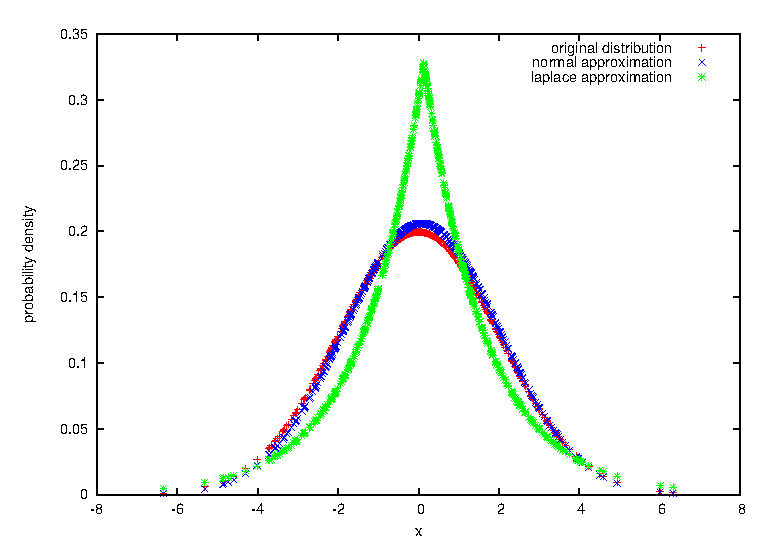
\includegraphics[width=0.45\textwidth]{fig/normal_n_500_mean_0_scale_2.eps}
        \label{fig:normal_data}
    }
    \hspace{0.5cm}
    \subfigure[Original distribution: Laplace]
    {
        \centering
        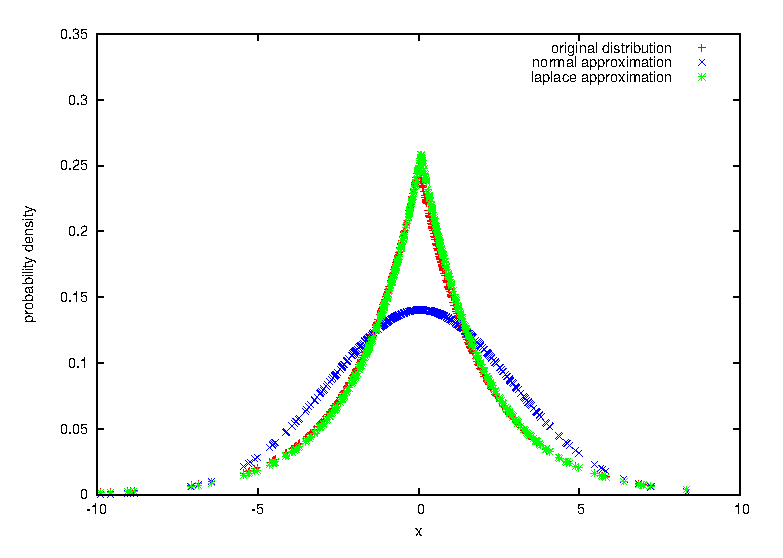
\includegraphics[width=0.45\textwidth]{fig/laplace_n_500_mean_0_scale_2.eps}
        \label{fig:laplace_data}
    }
    \caption{Approximation of data using Normal \& Laplace distributions}
    \label{fig:data_approximation}
\end{figure}

\begin{table}[h]
\centering
\caption{Comparison of the estimates (for a single iteration)}
\label{tab:comparison_estimates}
\begin{tabular}{|c|c|c|c|c|c|c|c|c|}
\hline
True & True & True & \multicolumn{3}{c|}{Normal estimates} & \multicolumn{3}{c|}{Laplace estimates} \\ \cline{4-9} 
distribution & mean & spread & mean & spread & msglen & mean & spread & msglen \\ \hline 
Normal & 0 & 2 & \multicolumn{1}{|r|}{-0.00687} & 1.92919 & \textbf{6491.21} & 0.0269173 & 1.56037 & 6535.04 \\ \hline
Laplace & 0 & 2 & \multicolumn{1}{|r|}{0.06303} & 2.84256 & 6770.24 & 0.0789925 & 1.93187 & \textbf{6688.78} \\ \hline
\end{tabular}
\end{table}

\begin{figure}[!htb]
  \centering
    \subfigure[Original distribution: Normal]
    {
      \centering
        \includegraphics[width=0.45\textwidth]{fig/statistics_normal_n_500_mean_0_scale_2.eps}
        \label{fig:normal_data_iterations}
    }
    \hspace{0.5cm}
    \subfigure[Original distribution: Laplace]
    {
        \centering
        \includegraphics[width=0.45\textwidth]{fig/statistics_laplace_n_500_mean_0_scale_2.eps}
        \label{fig:laplace_data_iterations}
    }
    \caption{Comparison of message lengths over 100 iterations}
    \label{fig:data_approximation_iterations}
\end{figure}

\autoref{fig:data_approximation_iterations} compares the message lengths over 100 iterations.
Each iteration involves generating 500 random data samples and modelling using both
distributions. For each iteration, there will be a message length corresponding to 
each of the distributions. In \ref{fig:normal_data_iterations}, the original 
distribution is Normal and it is observed
that over all the iterations, the message length for the Normal (red) is consistently less than that
of the Laplace (blue). A similar but reversed behaviour is observed when the data was generated
using the Laplace distribution as can be seen in \ref{fig:laplace_data_iterations}.
%In \autoref{fig:laplace_data_iterations}, the original distribution is 
%Laplace and it is observed that over all the iterations, the message length for the Laplace (blue) 
%is consistently less than that of the Normal (red).

\subsection{Superposition of vector sets}
Given any two vector sets $U = \{u_1,u_2,\ldots,u_m\}$ and $V = \{v_1,v_2,\ldots,v_m\}$
where each $u_i$ and $v_i (i \in \{1,2,\ldots,m\})$ is a vector in 3D space, the 
superpositioning problem refers to finding a suitable transformation on $U$ to
align it with $V$ such that the deviations of each vector in $V$ with its counterpart
in $U$ is minimized. Let the transformation be effected by a translation vector $t$ and a rotation matrix $R$.
Let it result in an altered vector set $U'=\{u_1',u_2',\ldots,u_m'\}$, where $u_i'=R(u_i-t)$.
Both the objective functions corresponding to the sum of squares ($\ell_2$ norm) of all deviations
\begin{equation} 
  \sum_{i=1}^m \|v_i-u_i'\|^2 = \sum_{i=1}^m \|v_i-R(u_i-t)\|^2 \label{eqn:L2_objective_function}
\end{equation} 
and the objective function corresponding to the sum of absolute deviations ($\ell_1$ norm)
\begin{equation} 
  \sum_{i=1}^m \|v_i-u_i'\| = \sum_{i=1}^m \|v_i-R(u_i-t)\| \label{eqn:L1_objective_function}
\end{equation}
(where $\|.\|$ denotes the vector norm) need to be minimized. 
The superposition problem can be formulated in the MML framework as finding the 
orientation of two proteins such that the deviations of each corresponding point
are encoded in an effective manner. Superposition based on minimizing total least
squares corresponds to stating the deviations using a Normal distribution. 
Superposition based on minimizing the absolute value of the deviations correspond
to transmitting the deviations using a Laplace distribution. \citet{keynes-laplace} 
showed that the Laplace distribution minimized the absolute deviation from the median
(which is also corroborated by the MML estimate of Laplace parameters 
\eqref{eqn:laplace_estimate}) and is, hence, pertinent for our current discussion. 

Minimization of \eqref{eqn:L2_objective_function} yields $t = \left(\frac{\sum_{i=1}^m u_i}{m} - \frac{R\sum_{i=1}^m v_i}{m}\right)$.
Substituting this value of $t$ in \eqref{eqn:L2_objective_function} results in the modified objective function:
\begin{equation}
\sum_{i=1}^m \left|\left|\left(v_i - \frac{\sum_{i=1}^m v_i}{m}\right) - R \left(u_i - \frac{\sum_{i=1}^m u_i}{m}\right)\right|\right|^2 \label{eqn:L2_after_translation}
\end{equation} 

\citet{kearsley89} provides a solution to \eqref{eqn:L2_objective_function} by 
resolving the transformation into translation and rotation. The centres of mass of the
two vector sets are translated to the origin \eqref{eqn:L2_after_translation} and the problem then reduces to finding the
rotation matrix which minimizes the total least squares. This involves respresenting
the rotation matrix using a quaternion and then solving the resultant eigenvalue 
decomposition problem. As such, \citet{kearsley89} offers an analytical way to solve
the \emph{least squares} superposition problem. 
 
Minimizing \eqref{eqn:L1_objective_function}, however, does not yield a closed form solution. 
Differentiating \eqref{eqn:L1_objective_function} with respect to $t$ and setting it to $0$ yields
\begin{equation}
\sum_{i=1}^m \frac{Rv_i-(u_i-t)}{\|Rv_i-(u_i-t)\|} = 0 \label{eqn:L1_after_translation}
\end{equation} 
In this case, $R$ and $t$ cannot be separated and, hence, an analytic solution does not exist. 
As such, one needs to resort to approximate methods to find the best $\ell_1$ superposition.
The one used in this paper is based on Monte Carlo simulation. 
It is described below:
\begin{enumerate}
\item Apply Kearsley's transformation and find the superposition that corresponds
to least sum of squares of the deviations. In this state, the value of the 
objective function \eqref{eqn:L1_objective_function} is computed. 
\item From this orientation, the protein is perturbed randomly. If the new orientation
results in a better value of the L1 norm \eqref{eqn:L1_objective_function}, the new orientation is
accepted. If however, the value of the objective function is less than the previous
value, the new orientation is accepted with a minute probability.
\item This is repeated for a certain number of iterations. The process is expected to converge to
the global minimum. As such, this would correspond to the optimal
superposition which minimizes the sum of absolute deviations.
\end{enumerate}

The two vector sets are first superposed using the Kearsley's method and the message
length ($I_{N}$) computed through MML inference using a Normal distribution. 
Monte Carlo simulation is performed (as discussed above) from this stage and
the final orientation is obtained. At this point, the message length ($I_L$) is
computed through MML inference using a Laplace distribution. Two cases arise:
\begin{itemize}
\item If $I_L < I_N$, then there exists a superposition that is better than the
one resulting from minimizing the sum of squared deviations \eqref{eqn:L2_objective_function}.
\item If $I_N < I_L$, then the superposition obtained by minimizing
\eqref{eqn:L2_objective_function} is better. Since the minimal $\ell_1$ superposition
is obtained using a Monte Carlo simulation (which is terminated after a certain number
of iterations), it could also be possible that the optimal solution wasn't found.
\end{itemize}

The aim of this exercise is to show that not all vector sets have their
optimal superpositions dictated by minimizing sum of squared deviations. It also drives
home the use of MML estimators in determining the kind of superposition to be
considered. 

\subsection*{Results}
We apply the problem of superposition to protein structures. In this context, the vector sets
corresponds to the three dimensional coordinates of the $\alpha$-carbon atoms of 
amino acid residues constituting the proteins' backbone. We use SUPER \citep{super}
(an implementation of Kearsley's orthogonal superposition)
to get all protein segments from the Protein Data Bank which fit to a Root Mean 
Squared Deviation (RMSD) of 5 Angstroms (\AA) or better. The protein segment corresponding
to PDB ID 2IC7, chain A and residues 132-162. This protein segment was randomly
considered and there were $\sim$23000 segments which fit within a RMSD of 5 \AA. 
The message length corresponding to this optimal $\ell_2$ superposition is calculated
using \eqref{eqn:normal_mml_estimate}. This orientation will also have a certain
value for the sum of absolute deviations. The message length to encode these
absolute differences is computed using \eqref{eqn:laplace_mml_estimate}.
For these 23000 segments across several proteins, we determine the optimal $\ell_1$ superposition
using our Monte Carlo simulation. The superposition resulting after 1000 iterations
is regarded as the optimal $\ell_1$ superposition. The message length to encode the
absolute differences is computed. There were about $\sim$1700 instances where the
optimal $\ell_1$ superposition is better than the $\ell_2$ equivalent. 
The results of the Monte Carlo simulation are shown in \autoref{tab:comparison_mml}. 

Each time we superimpose some protein segment with that of 2IC7, the other segment
is treated as a `fixed structure' and 2IC7 segment is randomly perturbed
from its optimal $\ell_2$ superposition. Each segment in the other protein 
is uniquely identified by its chain ID and residue span. These are obtained using SUPER.
RMSD is the error of fit of the $\ell_2$ superposition. The initial/final
$\ell_1$ deviations correspond to the average of the absolute deviations
in both these orientations;
msglen($\ell_2$) is the message length using a Normal distribution to encode the
deviations in the optimal $\ell_2$ superposition; msglen (initial $\ell_1$) corresponds to the
message length of encoding the absolute deviations before perturbations and msglen (final $\ell_1$)
is the message length to encode the deviations after the Monte Carlo simulation.
\begin{table}[ht]
\centering
\caption{Comparison of the minimum message lengths}
\label{tab:comparison_mml}
\begin{tabular}{|c|c|c|c|c|c|c|}
\hline
Fixed & RMSD & Initial $\ell_1$ & Final $\ell_1$ & msglen & msglen & msglen \\
structure & (in \AA) & deviation (in \AA) & deviation (in \AA) & ($\ell_2$) & (initial $\ell_1$) & (final $\ell_1$) \\
\hline
3IGJ [A:139-169] & 1.834 & 1.910 & 1.872 & 1134.82 & 1102.03 & \textbf{1100.28} \\
4G87 [A:291-321] & 2.112 & 2.555 & 2.465 & 1153.54 & 1165.38 & \textbf{1138.59} \\
3R2W [B:435-465] & 3.437 & 4.637 & 4.593 & \textbf{1218.17} & 1228.74 & 1222.79 \\
\hline
\end{tabular}
\end{table}
As expected, the final $\ell_1$ deviation is less than the initial one. It is observed this happens for 
most of the cases which suggest the presence of the $\ell_1$ optimum somewhere close
to the initial position. 

For the discussion below, in \autoref{fig:compare_structure_1}, \ref{fig:compare_structure_2},
\ref{fig:compare_structure_3}, the red curve corresponds to the fixed protein; the blue curve
is the optimal $\ell_2$ superposition (of the 2IC7 segment), and the green curve corresponds to its 
optimal $\ell_1$ superposition.

The first row in \autoref{tab:comparison_mml} corresponds to \autoref{fig:compare_structure_1}.
Its msglen(initial $\ell_1$) $<$ msglen($\ell_2$). This suggests that $\ell_1$ superposition supercedes 
the $\ell_2$ superposition, and it only gets better
as the structure is perturbed as is evidenced by msglen(final $\ell_1$) -- the message length
after the Monte Carlo simulation. Here, it can be seen that the red curve (the fixed protein) 
is closer to the green curve ($\ell_1$ superposition) than to the blue curve ($\ell_2$ superposition)
in the majority of the protein structure.
\begin{figure}[!htb]
\centering
\includegraphics[scale=0.5]{fig/compare_structure_1.eps}
%\caption{Initial \& final $\ell_1$ superposition better than $\ell_2$ superposition}
\caption{Stereo images of the superposition of segments from 2IC7 (red) \& 3IGJ (fixed). Initial \& final $\ell_1$ superposition (green) better than $\ell_2$ superposition (blue).}
\label{fig:compare_structure_1}
\end{figure}
\begin{figure}[!htb]
  \centering
    \subfigure[Final $\ell_1$ superposition (green) better than $\ell_2$ superposition (blue)]
    {
      \centering
        \includegraphics[width=0.45\textwidth]{fig/compare_structure_2.eps}
        \label{fig:compare_structure_2}
    }
    \hspace{0.5cm}
    \subfigure[$\ell_2$ superposition (blue) better than $\ell_1$ superposition (green)]
    {
        \centering
        \includegraphics[width=0.45\textwidth]{fig/compare_structure_3.eps}
        \label{fig:compare_structure_3}
    }
    \caption{Comparing the protein superpositions with respect to $\ell_1$ and $\ell_2$ norm}
    \label{fig:protein_superposition}
\end{figure}

The second row in \autoref{tab:comparison_mml} corresponds to the case where the final $\ell_1$
superposition (1138.59 bits) is better than the $\ell_2$ superposition (1153.54 bits). The initial
$\ell_1$ superposition (1165.38 bits) is not the optimal one and hence, the 
Monte Carlo simulation goes through a series of
iterations to reach the local optimum. In \ref{fig:compare_structure_2}, the red curve is closer
to the  green curve (final $\ell_1$) than to the blue curve ($\ell_2$ superposition).
%\begin{figure}[!htb]
%\centering
%\includegraphics[scale=0.5]{fig/compare_structure_2.eps}
%\label{fig:compare_structure_2}
%\caption{Final $\ell_1$ superposition better than $\ell_2$ superposition}
%\end{figure}
The third row in \autoref{tab:comparison_mml} demonstrates the case where the $\ell_2$ superposition
(1218.17 bits) is optimal compared to the $\ell_1$ superposition (1222.79 bits). On careful 
inspection, one can see that the red curve (in \ref{fig:compare_structure_3}) is closer
to the blue curve corresponding to the $\ell_2$ superposition than to the green curve (the optimal $\ell_1$ superposition).
%\begin{figure}[!htb]
%\centering
%\includegraphics[scale=0.5]{fig/compare_structure_3.eps}
%\label{fig:compare_structure_3}
%\caption{$\ell_2$ superposition better than $\ell_1$ superposition}
%\end{figure}

\section{Conclusion}
We have derived the MML estimators for the Laplace distribution and applied them
in the context of encoding the superposition of vector sets. This is used to
distinguish the quality of superposition for any two vector sets. 
In general, if the objective function is formulated as the sum of absolute differences,
we have a framework using MML to encode these values using 
a Laplace distribution. The quality of the overall fit can be evaluated using the
MML inference technique and can be compared with other models.
For the specific problem of superposition of two vector sets, the choice of $\ell_1$ or $\ell_2$
superposition is made by comparing the message lengths obtained by encoding deviations
using $\ell_1$ and $\ell_2$ norm.

\acks{We thank Arun Konagurthu for the numerous discussions we had regarding the superposition application. We also thank Maria Garcia de la Banda and James Collier for proof reading the paper.} 

\bibliography{references}

\appendix
\section{Derivations involved in the computation of Laplace Fisher}
\label{apd:laplace_fisher}
\begin{align*}
 \frac{\partial L}{\partial \mu} &= -\frac{1}{b} \sum_{n=1}^N \frac{(x_n-\mu)}{|x_n-\mu|} \quad\quad\left(\mathrm{using} \frac{d}{dx}|x| = \frac{d}{dx}\sqrt{x^2} = \frac{x}{|x|}\right)
\end{align*}
This is discontinuous as it is piecewise constant. Hence to calculate $\frac{\partial^2 L}{\partial \mu^2}$, the following approach is adopted.
Assume that the actual distribution has parameters $m$ and 
$b$. The receiver, however, decodes the mean as $\mu$ to an accuracy of parameter
value $\delta$. As such $\mu$ is a random variable and it is fair to assume 
that $\mu \in \left[m-\frac{\delta}{2},m+\frac{\delta}{2}\right]$. I_1t is 
assumed that $\mu$ follows a uniform distribution in this range. Using this 
assumption, now we compute the $\mathrm{E}\left[\frac{\partial L}{\partial \mu}\right]$ 
and subsequent calculations. From our assumptions, $\mathrm{pdf}(\mu) = \frac{1}{\delta}$.
\begin{align*}
 \mathrm{Therefore,}\quad \frac{\partial L}{\partial \mu} &\approx \mathrm{E}\left[\frac{\partial L}{\partial \mu}\right] = -\frac{1}{b}\mathrm{E}\left[\sum_{n=1}^{N}\frac{x_n-\mu}{|x_n-\mu|}\right]
\end{align*}
\begin{align*}
 \mathrm{E}\left[\frac{x-\mu}{|x-\mu|}\right] &= \int\limits_{-\infty}^{\infty} \frac{x-\mu}{|x-\mu|}.\frac{1}{2b}.e^{\frac{|x-m|}{b}} dx \\
 &= \int\limits_{-\infty}^{\mu} -\frac{1}{2b} e^{-\frac{|x-m|}{b}} dx + \int\limits_{\mu}^{\infty} \frac{1}{2b} e^{-\frac{|x-m|}{b}} dx
\end{align*}
(i) Let $\mu < m$
\begin{align*}
 \mathrm{Therefore,}\quad \mathrm{E}\left[\frac{x-\mu}{|x-\mu|}\right] &= \int\limits_{-\infty}^{\mu} -\frac{1}{2b} e^{\frac{x-m}{b}} dx + \int\limits_{\mu}^{m} \frac{1}{2b} e^{\frac{x-m}{b}} dx + \int\limits_{m}^{\infty} \frac{1}{2b} e^{-\frac{x-m}{b}} dx \\
 &= 1 - e^{\frac{\mu-m}{b}}
\end{align*}
(ii) Let $\mu > m$
\begin{align*}
 \mathrm{Therefore,}\quad \mathrm{E}\left[\frac{x-\mu}{|x-\mu|}\right] &= \int\limits_{-\infty}^{m} -\frac{1}{2b} e^{\frac{x-m}{b}} dx + \int\limits_{m}^{\mu} -\frac{1}{2b} e^{-\frac{x-m}{b}} dx + \int\limits_{\mu}^{\infty} \frac{1}{2b} e^{-\frac{x-m}{b}} dx \\
 &= -(1 - e^{-\frac{\mu-m}{b}})
\end{align*}
(i) and (ii) can be merged and hence, $\mathrm{E}\left[\frac{x-\mu}{|x-\mu|}\right] = - sgn(\mu-m) (1 - e^{-\frac{|\mu-m|}{b}})$. From the argument above,
\begin{align}
 \frac{\partial L}{\partial \mu} &\approx \mathrm{E}\left[\frac{\partial L}{\partial \mu}\right] = -\frac{1}{b} \mathrm{E}\left[\sum_{n=1}^{N}\frac{x_n-\mu}{|x_n-\mu|}\right]\notag\\
 &= \frac{N}{b} sgn(\mu-m) (1 - e^{-\frac{|\mu-m|}{b}}) \label{eqn:laplace_expected_approx}\\
 \mathrm{Therefore,}\quad \frac{\partial^2 L}{\partial \mu^2} &= \frac{N}{b^2} e^{\frac{-|\mu-m|}{b}} \notag\\
 \mathrm{E} \left[\frac{\partial^2 L}{\partial \mu^2}\right] &= \frac{N}{b^2} \mathrm{E}\left[e^{\frac{-|\mu-m|}{b}}\right] \notag
\end{align}
\begin{align*}
 \mathrm{E}\left[e^{\frac{-|\mu-m|}{b}}\right] &= \int\limits_{m-\frac{\delta}{2}}^{m+\frac{\delta}{2}} e^{\frac{-|\mu-m|}{b}} . \frac{1}{\delta} . d\mu \\
 &= \frac{1}{\delta} \int\limits_{m-\frac{\delta}{2}}^{m} e^{\frac{\mu-m}{b}} d\mu + \int\limits_{m}^{m+\frac{\delta}{2}}e^{-\frac{\mu-m}{b}} d\mu \\
 &= 2b \left(\frac{1-e^{-\frac{\delta}{2b}}}{\delta}\right) \\
 &= 2b \left( \frac{1}{2b} - \frac{1}{2b}\mathcal{O}\left(\frac{\delta}{2b}\right) \right) \quad\quad(\mathrm{assuming} \quad \delta \ll 2b) \\
 &\approx 1
 \end{align*}
\begin{equation*}
 \mathrm{Therefore,}\quad \mathrm{E} \left[\frac{\partial^2 L}{\partial \mu^2}\right] = \frac{N}{b^2} (1) = \frac{N}{b^2}
\end{equation*}
Using \eqref{eqn:laplace_expected_approx}, 
\begin{align*}
 \frac{\partial^2 L}{\partial b \partial \mu} &= N sgn(\mu-m) \left[ -\frac{1}{b^2} - \left( e^{\frac{-|\mu-m|}{b}} \left( -\frac{1}{b^2} \right) + \frac{1}{b} e^{\frac{-|\mu-m|}{b}} \frac{|\mu-m|}{b^2} \right) \right] \\
 &= -\frac{N}{b^2} sgn(\mu-m)(1-e^{-\frac{|\mu-m|}{b}}) - \frac{N}{b} . \frac{(\mu-m)}{b^2} . e^{-\frac{|\mu-m|}{b}} \\
 \mathrm{Therefore,}\quad \mathrm{E} \left[\frac{\partial^2 L}{\partial b \partial \mu}\right] &= -\frac{N}{b^2} (\mathrm{E}_1 - \mathrm{E}_2) - \frac{N}{b^3} \mathrm{E}_3, \quad\quad\mathrm{where}
\end{align*}
\begin{align*}
 \mathrm{E}_1 &= \mathrm{E}[sgn(\mu-m)] = \int\limits_{m-\frac{\delta}{2}}^{m+\frac{\delta}{2}} sgn(\mu-m).\frac{1}{\delta}.d\mu = \frac{1}{\delta} \int\limits_{m-\frac{\delta}{2}}^{m+\frac{\delta}{2}} \frac{\mu-m}{|\mu-m|} d\mu \\
 &= \frac{1}{\delta} \int\limits_{-\frac{\delta}{2}}^{\frac{\delta}{2}} \frac{t}{|t|} dt = 0 \quad\quad(\mathrm{as\,\,the\,\,integrand\,\,is\,\,an\,\,odd\,\,function})
\end{align*}
\begin{align*}
 \mathrm{E}_2 &= \mathrm{E}[sgn(\mu-m)e^{-\frac{|\mu-m|}{b}}] = \frac{1}{\delta} \int\limits_{m-\frac{\delta}{2}}^{m+\frac{\delta}{2}} \frac{\mu-m}{|\mu-m|} e^{-\frac{|\mu-m|}{b}} d\mu \\
 &= \frac{b}{\delta} \int\limits_{-\frac{\delta}{2}}^{\frac{\delta}{2}} \frac{t}{|t|} e^{-|t|} dt = 0 \quad\quad(\mathrm{as\,\,the\,\,integrand\,\,is\,\,an\,\,odd\,\,function})
\end{align*}
\begin{align*}
 \mathrm{E}_3 &= \mathrm{E}[(\mu-m)e^{-\frac{|\mu-m|}{b}}] = \frac{1}{\delta} \int\limits_{m-\frac{\delta}{2}}^{m+\frac{\delta}{2}} (\mu-m)e^{-\frac{|\mu-m|}{b}} d\mu \\
 &= \frac{b^2}{\delta} \int\limits_{-\frac{\delta}{2}}^{\frac{\delta}{2}} t e^{-|t|} dt = 0 \quad\quad(\mathrm{as\,\,the\,\,integrand\,\,is\,\,an\,\,odd\,\,function})
\end{align*}
\begin{equation*} 
  \mathrm{Therefore,}\quad \mathrm{E} \left[\frac{\partial^2 L}{\partial b \partial \mu}\right] = 0 
\end{equation*}

\end{document}

